% Chapter 2

\chapter{Notazioni e definizioni} % Chapter title

\label{ch:examples} % For referencing the chapter elsewhere, use \autoref{ch:examples} 

\begin{enumerate}
	
	\item \textit{GeoArea} : Definisce un territorio di interesse per il calcolo dell'esposizione a rischio frana. La \textit{GeoArea} può rappresentare un comune, una provincia (Figura \ref{RomaBoundary}), una regione (Figura \ref{LazioBoundary}), una nazione (Figura \ref{ItaliaBoundary}) fino ad arrivare ad un intero continente. GeoArea è descritta dalla tupla <\textit{ID}, \textit{description}, \textit{boundary}>.
	
	\begin{figure}[h]
		\hspace{0.02\linewidth}
		\begin{minipage}[t]{0.3\linewidth}
			\centering
			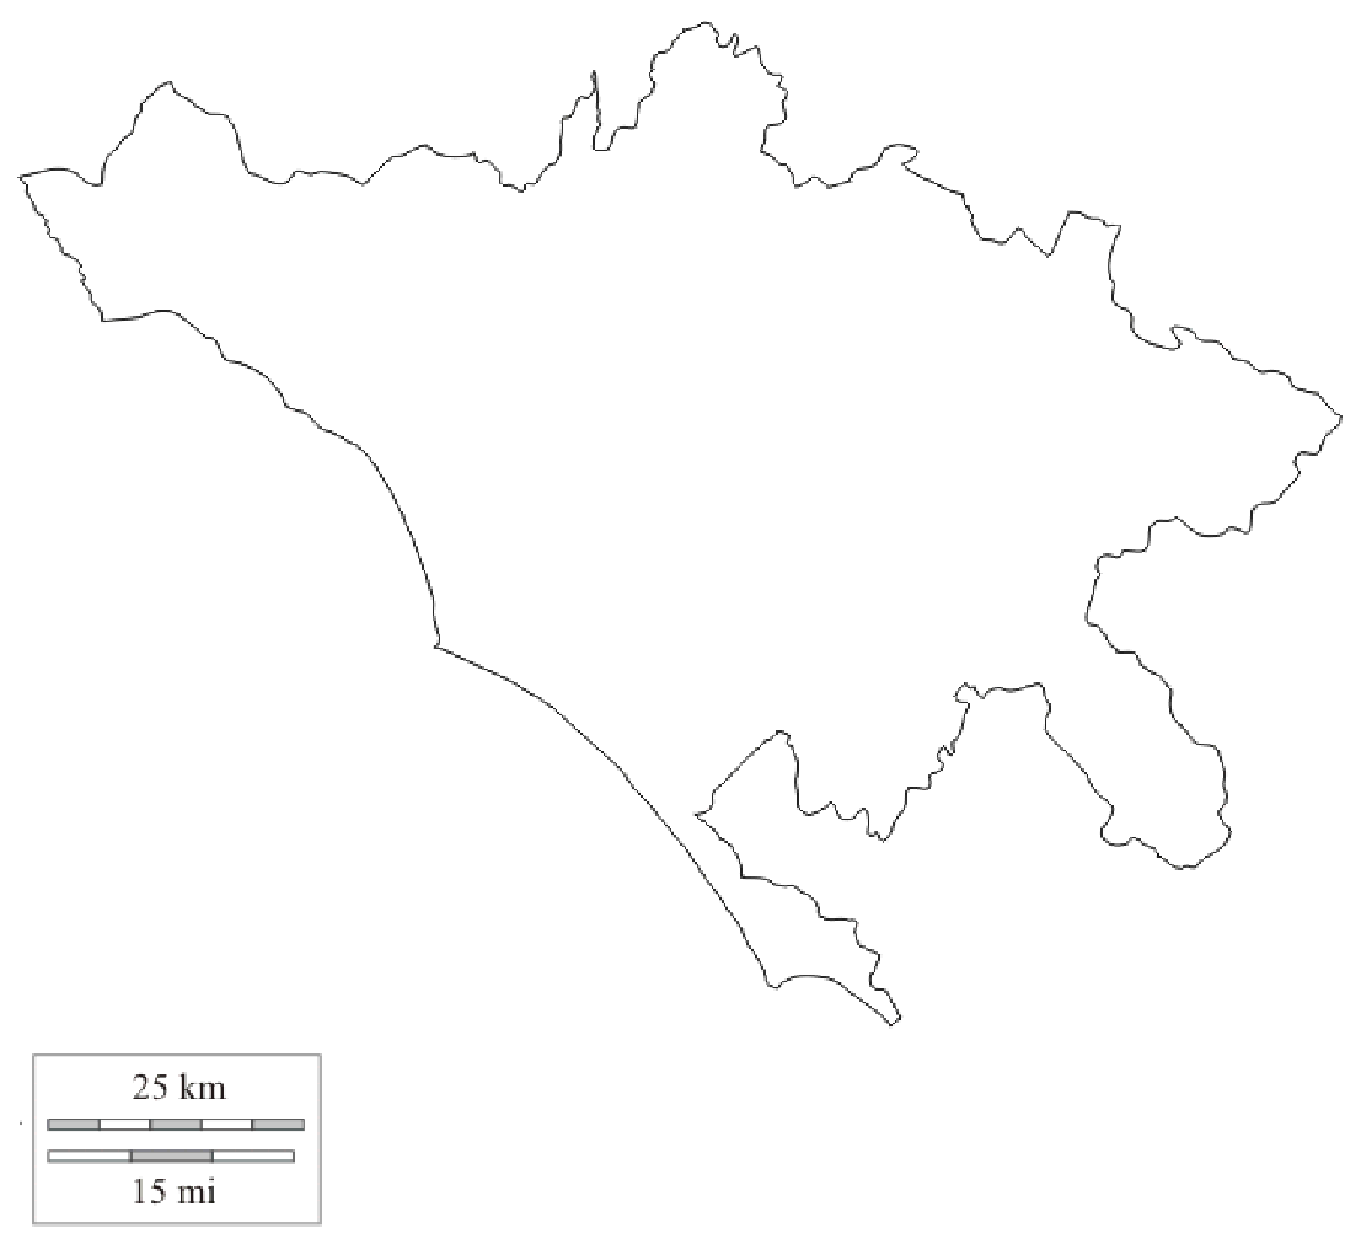
\includegraphics[width=1\textwidth]{images/roma}
			\caption{Confini della provincia di Roma.}
			\label{RomaBoundary}
		\end{minipage}
		\hspace{0.03\linewidth}
		\begin{minipage}[t]{0.3\linewidth}
			\centering
			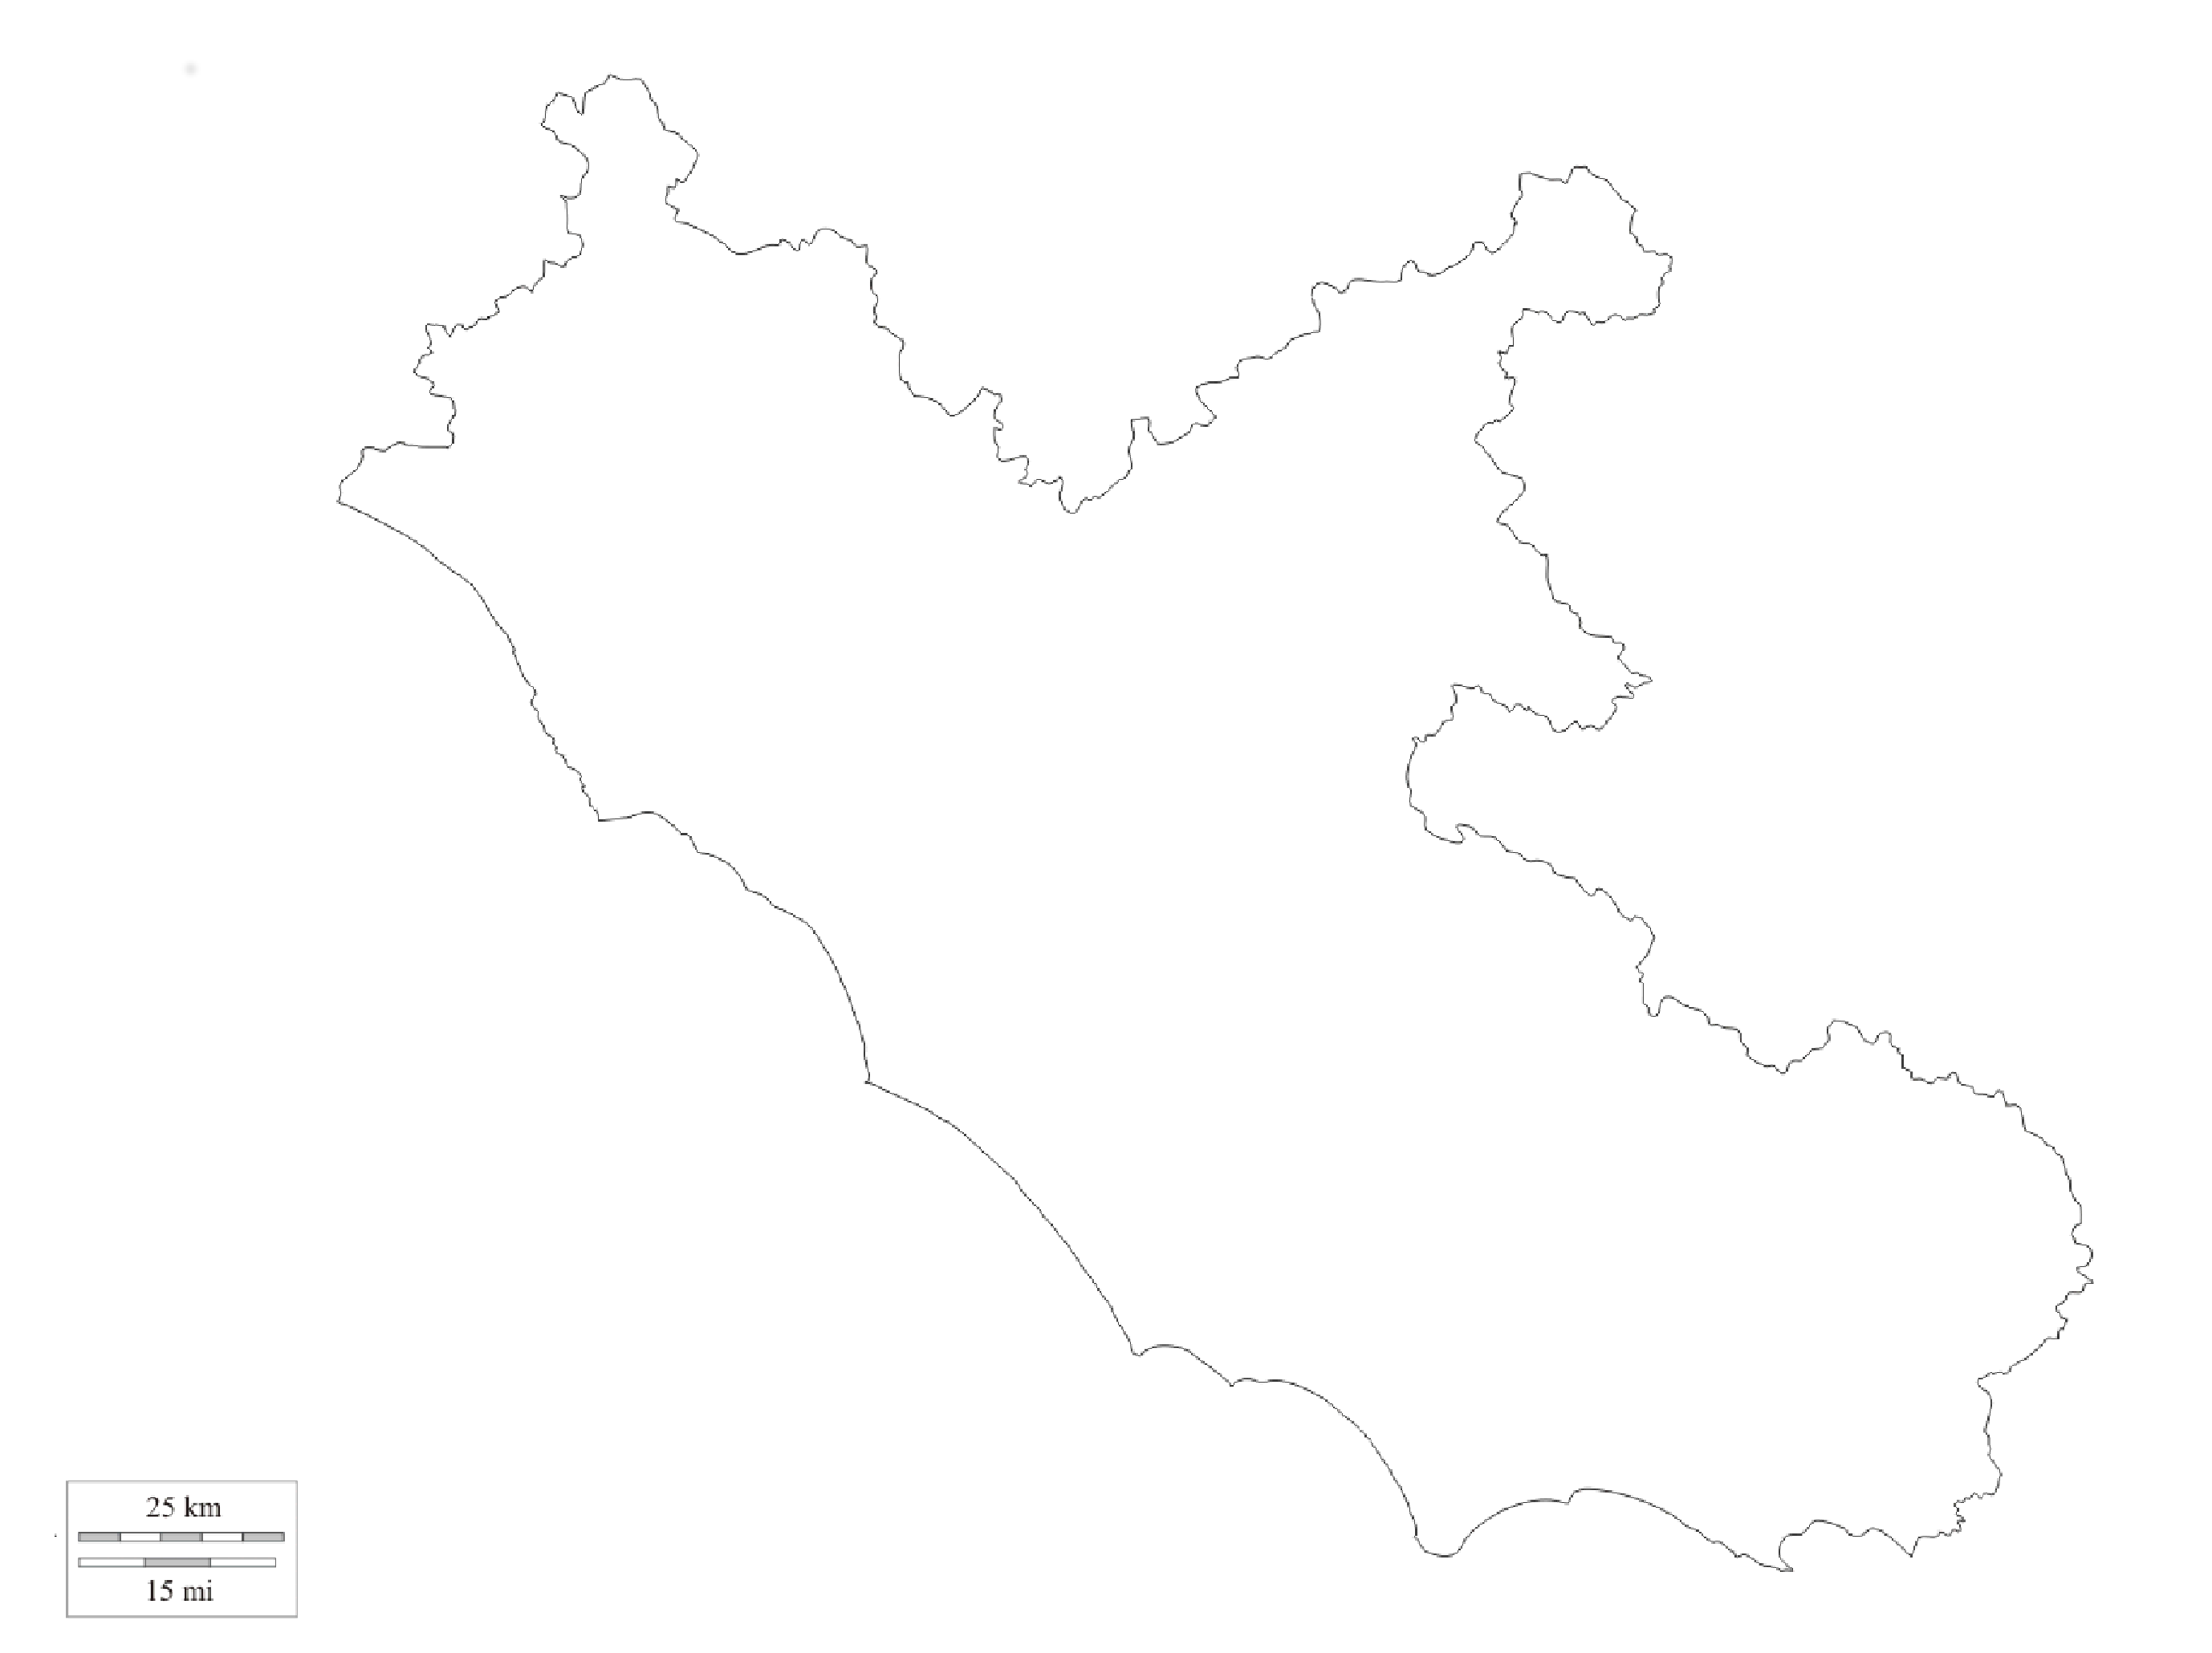
\includegraphics[width=1\textwidth]{images/lazio}
			\caption{Confini della regione Lazio.}
			\label{LazioBoundary}
		\end{minipage}
		\hspace{0.02\linewidth}
		\begin{minipage}[t]{0.3\linewidth}
			\centering
			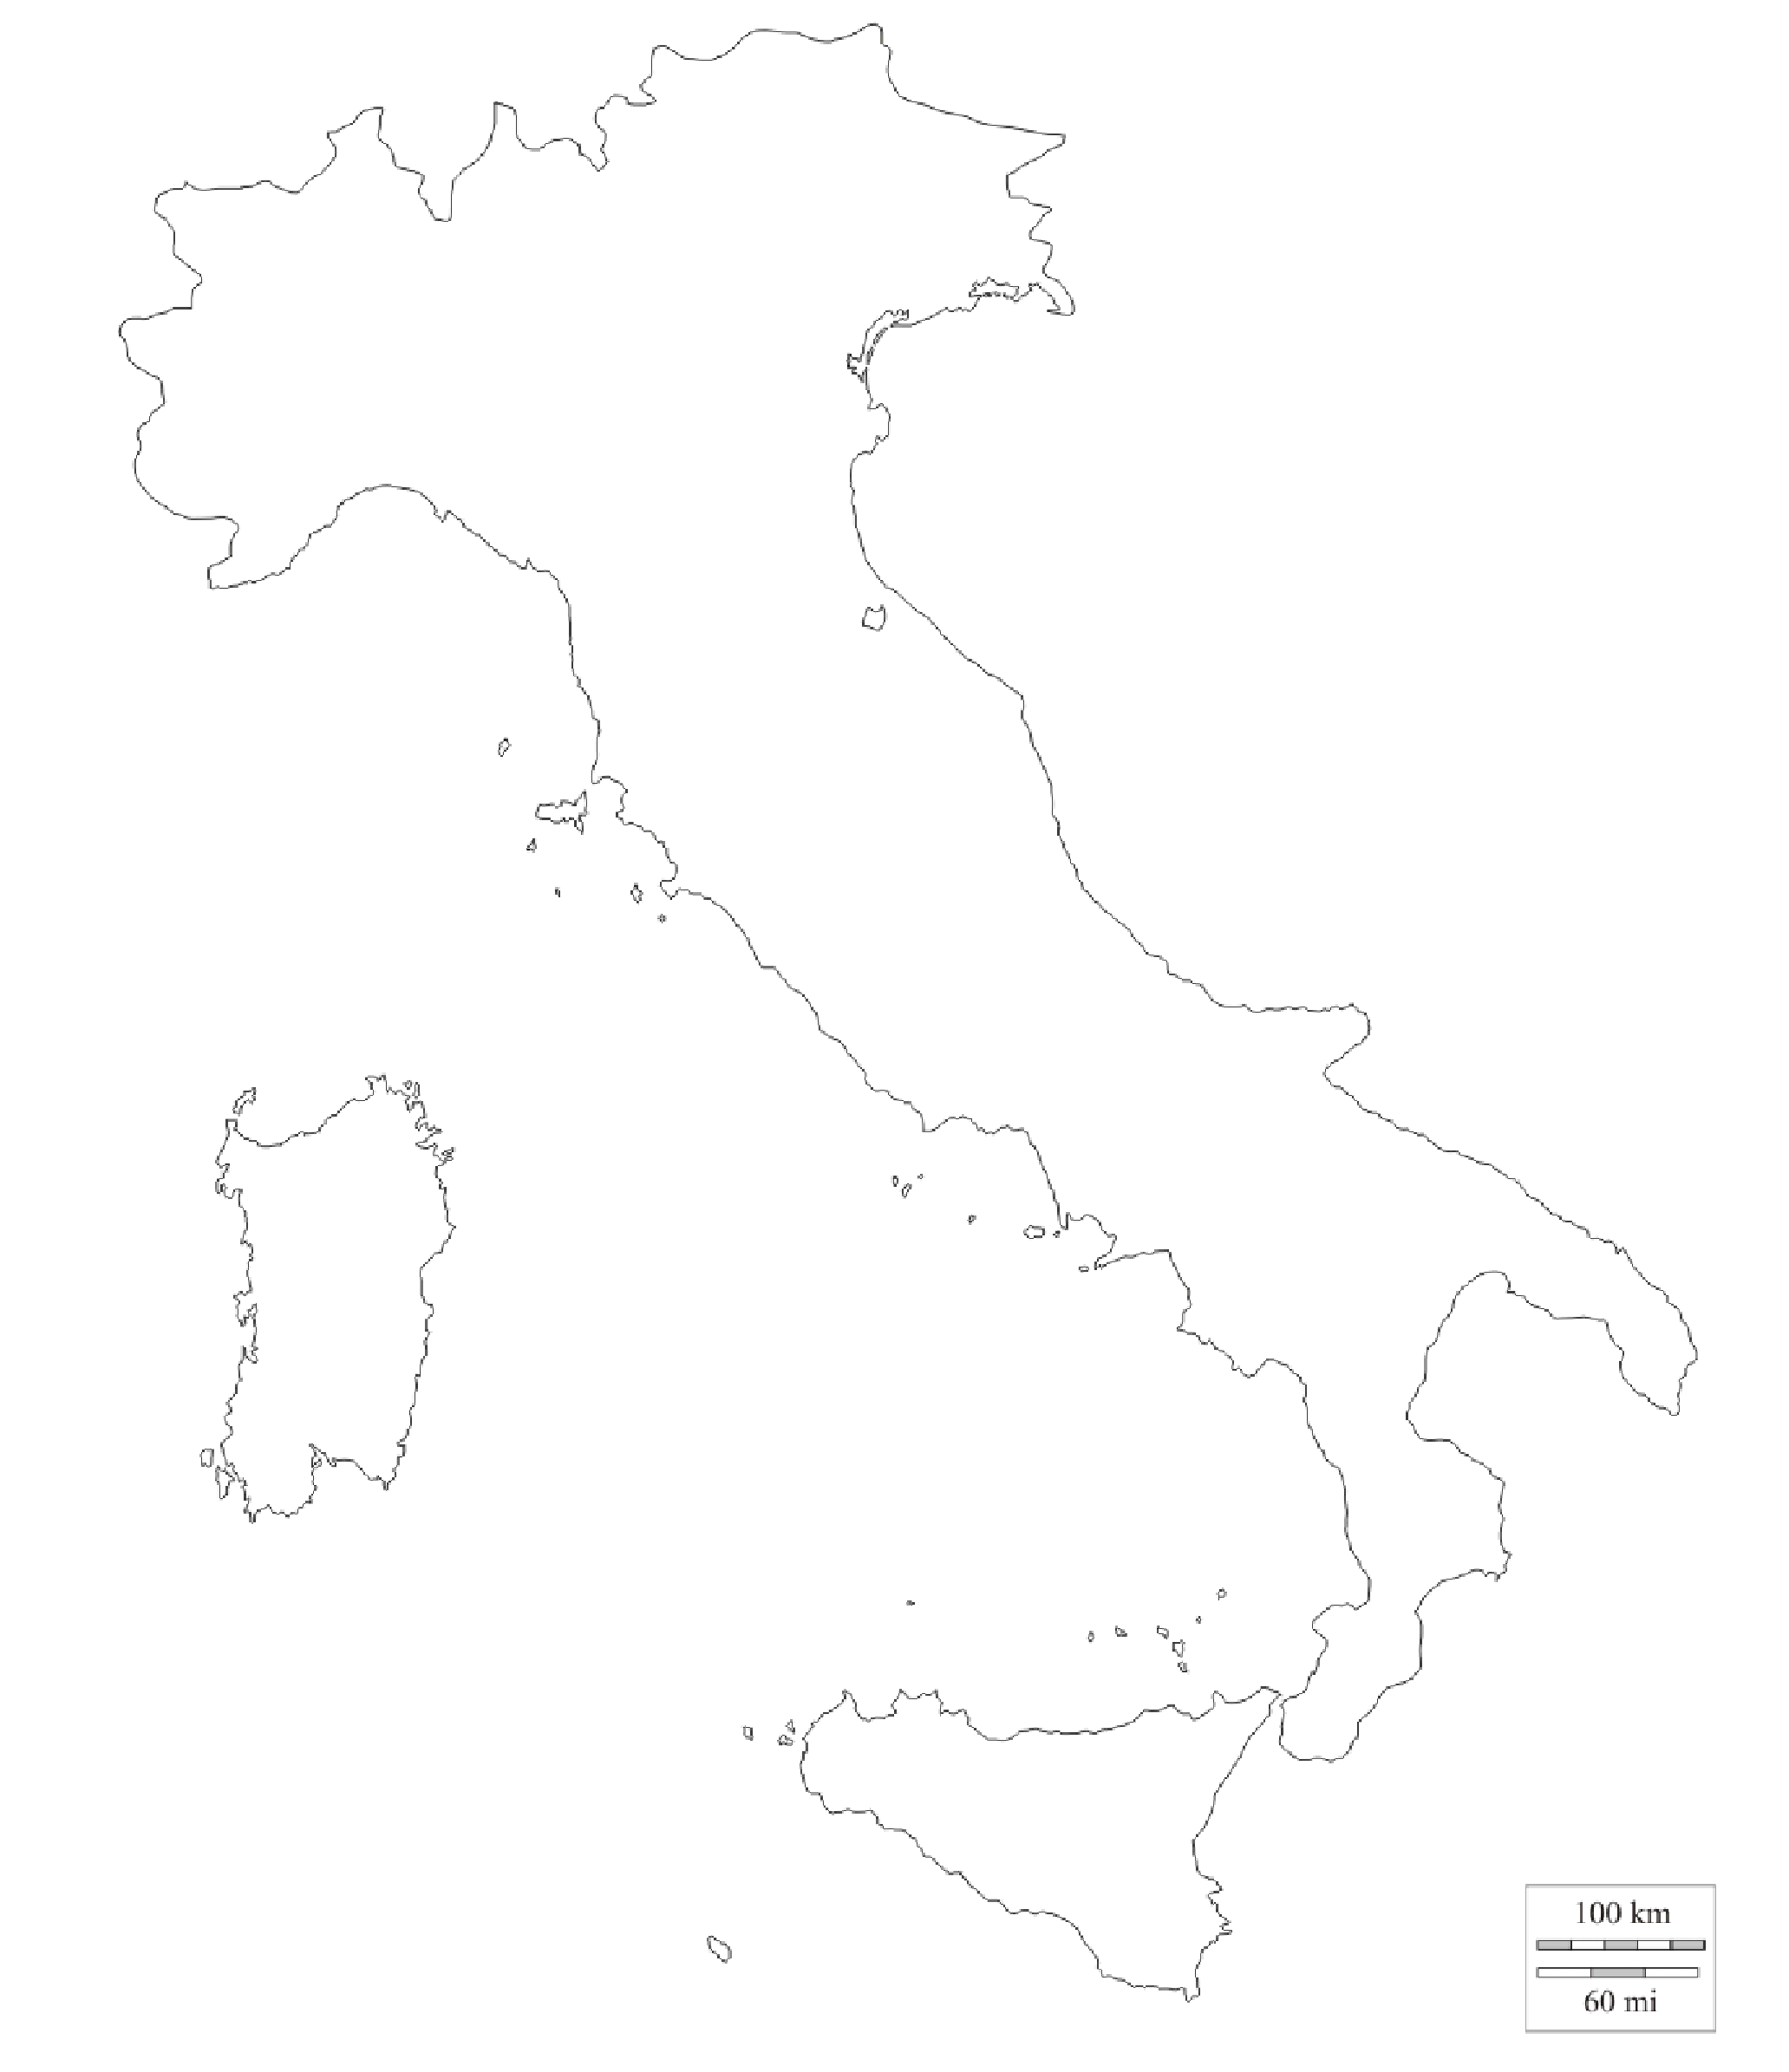
\includegraphics[width=1\textwidth]{images/italia}
			\caption{Confini del territorio italiano.}
			\label{ItaliaBoundary}
		\end{minipage}
	\end{figure}
	
	
	\item  \textbf{$ \mathcal{Z} $ (Zones)} $ = \{ z_k(k=1,2,..) | z_k $ \`e una \textit{Zone} di  GeoArea \}. Una \textit{Zone} definisce una porzione di terreno all'interno della GeoArea ed è descritta dalla tupla <\textit{ID}, \textit{boundary}, \textit{$Sz_k$}>. Il campo \textit{ID} identifica univocamente la k-esima \textit{Zone}, \textit{boundary} la geometria del confine e \textit{$Sz_k$} è un valore decimale che rappresenta la probabilità di frana di $z_k$ (Figura \ref{Zk}).
	Si noti che $zk$ è una notazione sovraccaricata in quanto rappresenta sia l’\textit{ID} di una \textit{Zone} che la sua geometria.
	
	\begin{figure}[h]
		\centering
		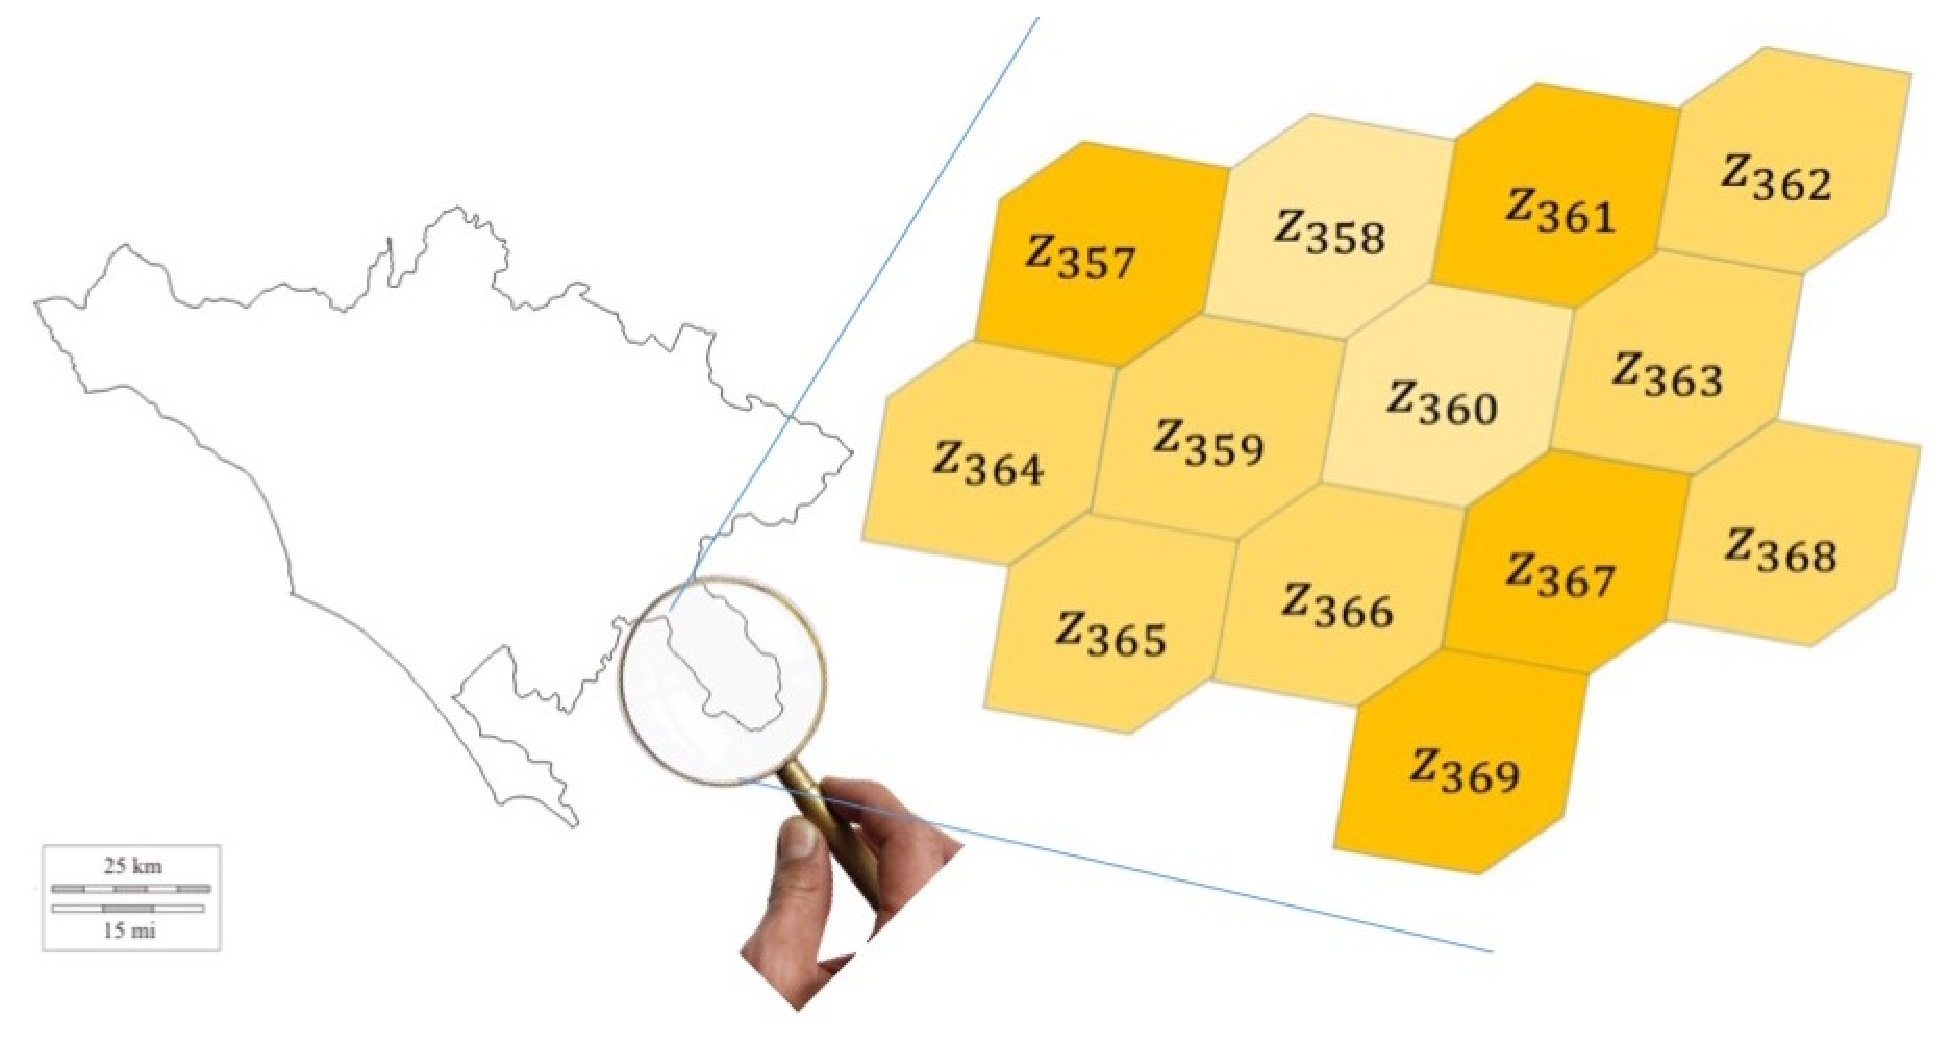
\includegraphics[width=0.7\textwidth]{images/zk}
		\caption{Rappresentazione delle Zones di una \textit{GeoArea}. La geometria del confine delle porzioni di terreno è puramente indicativa. Le diverse tonalità di arancione rappresentano i valori di $Sz_k$  delle \textit{Zones}.}
		\label{Zk}
	\end{figure}
	
	\item \textbf{$ \mathcal{B} $ (Buildings)} $ = \{b_i(i=1,2,..) | b_i $ è un \textit{building} ubicato all'interno dei confini della  GeoArea \}. Per building si intende un generico edificio (come ad esempio una scuola, un grattacielo, un hotel e strutture simili) descritto dalla tupla < \textit{ID}, \textit{description}, \textit{position}>. Il campo \textit{ID} identifica univocamente l'edificio; \textit{description} una sua descrizione testuale e infine \textit{position} rappresenta la posizione geografica di $ b_i $ espressa da una coppia di coordinate geografiche (Figura \ref{station}). Definiamo con $\mathbf{card}(\mathcal{B})$ la cardinalità dell'insieme $ \mathcal{B} $, ovvero il numero di edifici presenti in \textit{GeoArea}. Dettagli come la planimetria della struttura potrebbero fornire ulteriori dati sensibili ma sono molto difficili da reperire e quindi non verranno presi in considerazione.
	In seguito verrà usato sempre il pedice $i$ per riferirsi al building $i-esimo$.
	Nelle notazioni introdotte di seguito l'occorrenza del pedice $i$ viene usata $sempre$ per richiamare che ci si riferisce all'edificio $i-mo$, ovvero all'elemento $b_i$ di $ \mathcal{B} $.
	
	\item \textbf{$HazardArea_i$} rappresenta l'area a possibile rischio smottamento circostante l'edificio $b_i$, definita come la circonferenza centrata su $b_i$ di raggio $r$ (Figura \ref{buffer}).
	
	\begin{figure}[h]
		\hspace{0.1\linewidth}
		\begin{minipage}[t]{0.35\linewidth}
			\centering
			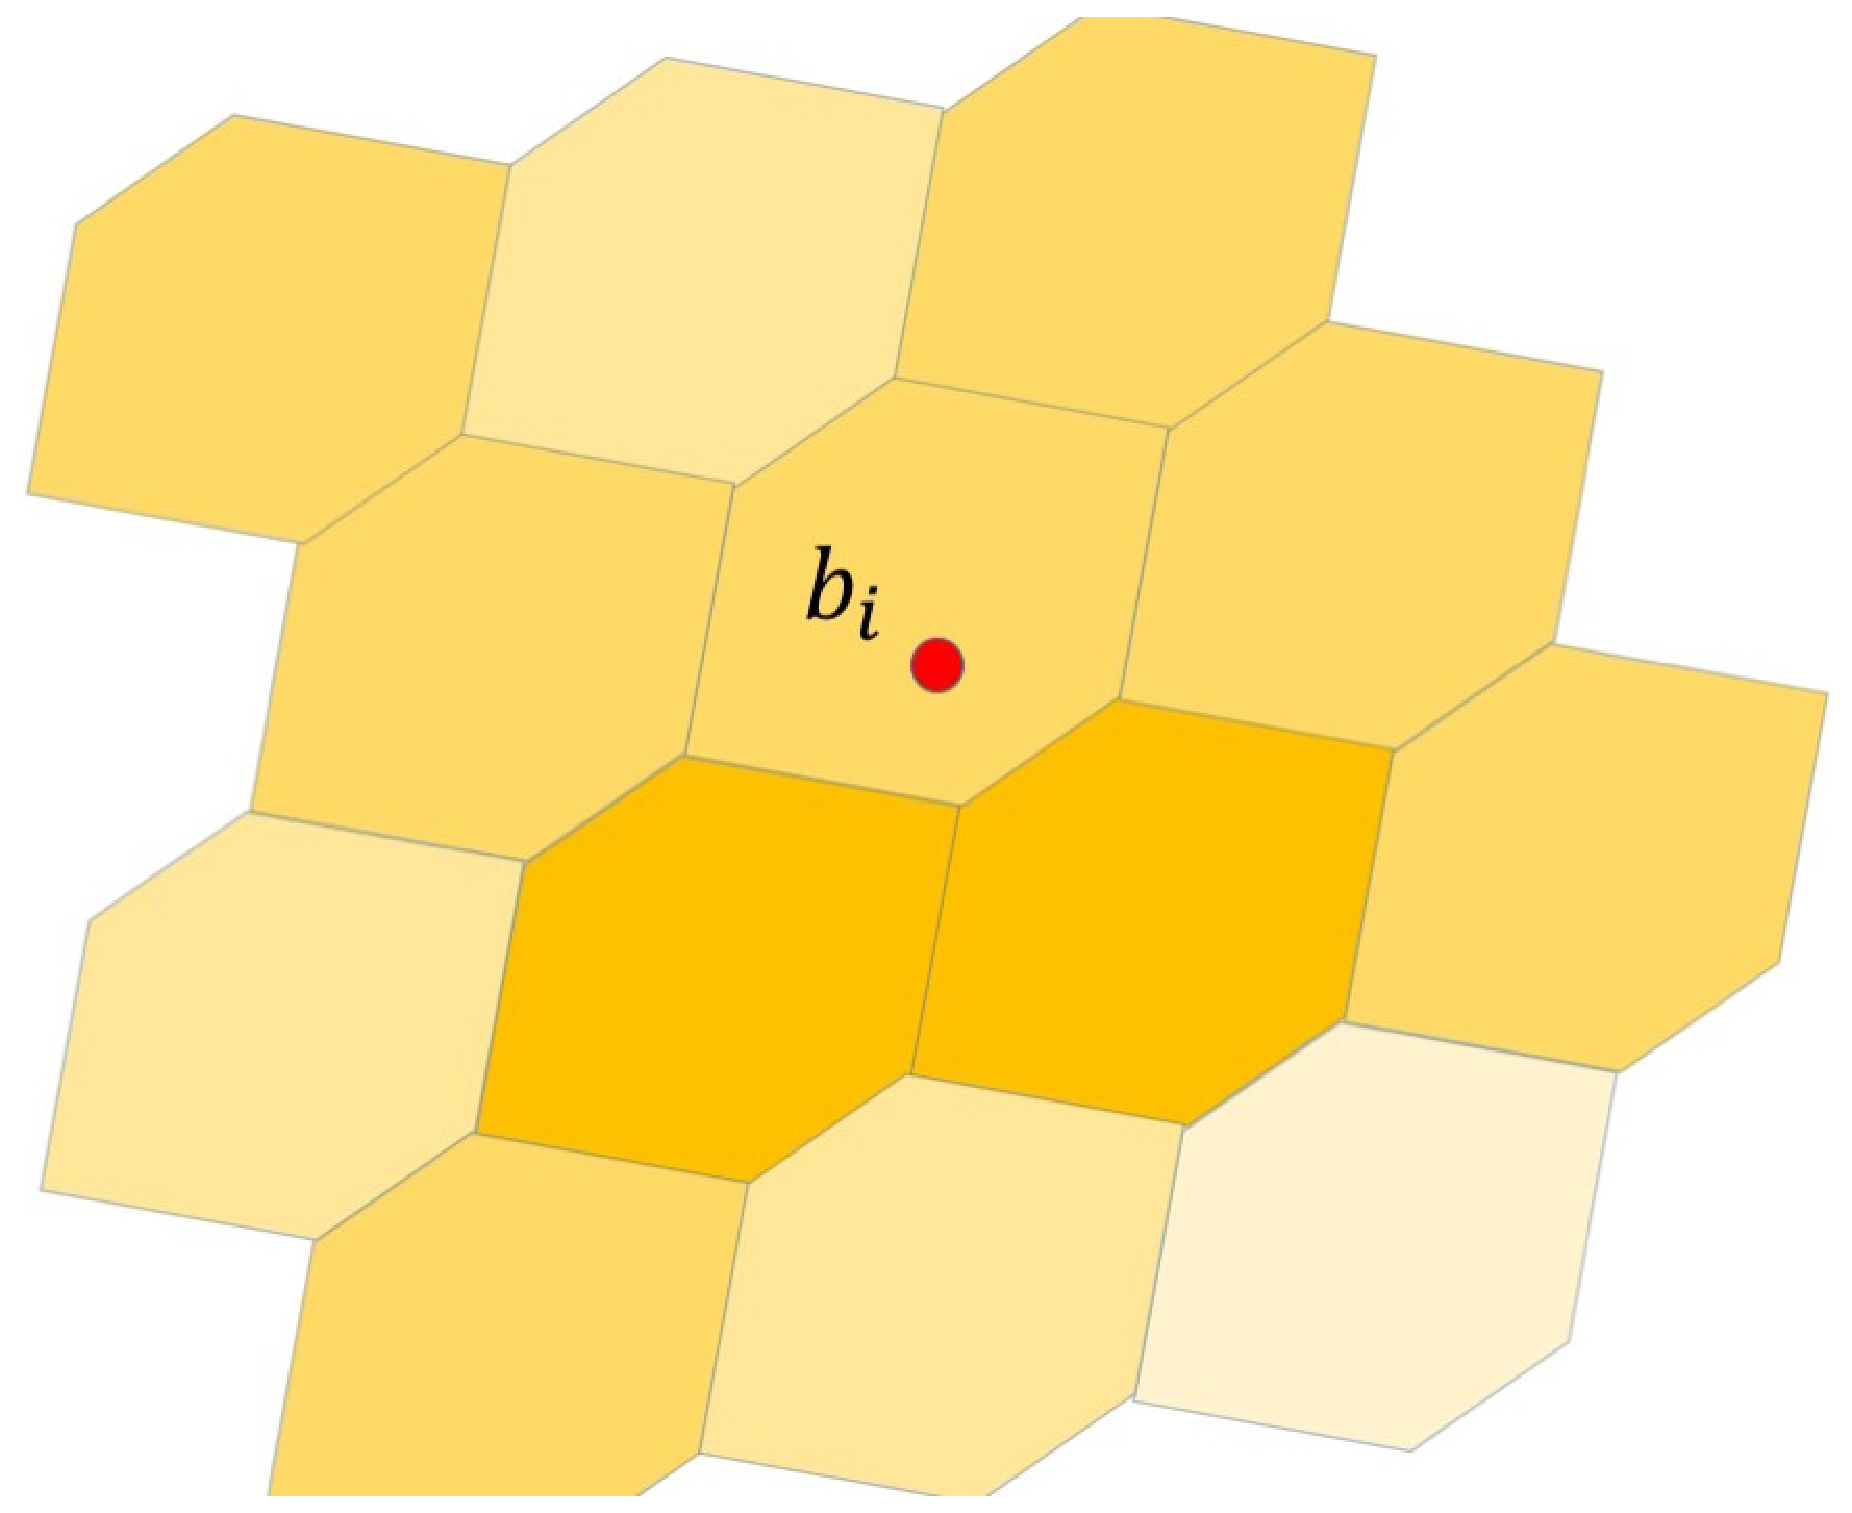
\includegraphics[width=1\textwidth]{images/station}
			\caption{Il pallino rosso rappresenta il generico edificio $b_i$.}
			\label{station}
		\end{minipage}
		\hspace{0.13\linewidth}
		\begin{minipage}[t]{0.35\linewidth}
			\centering
			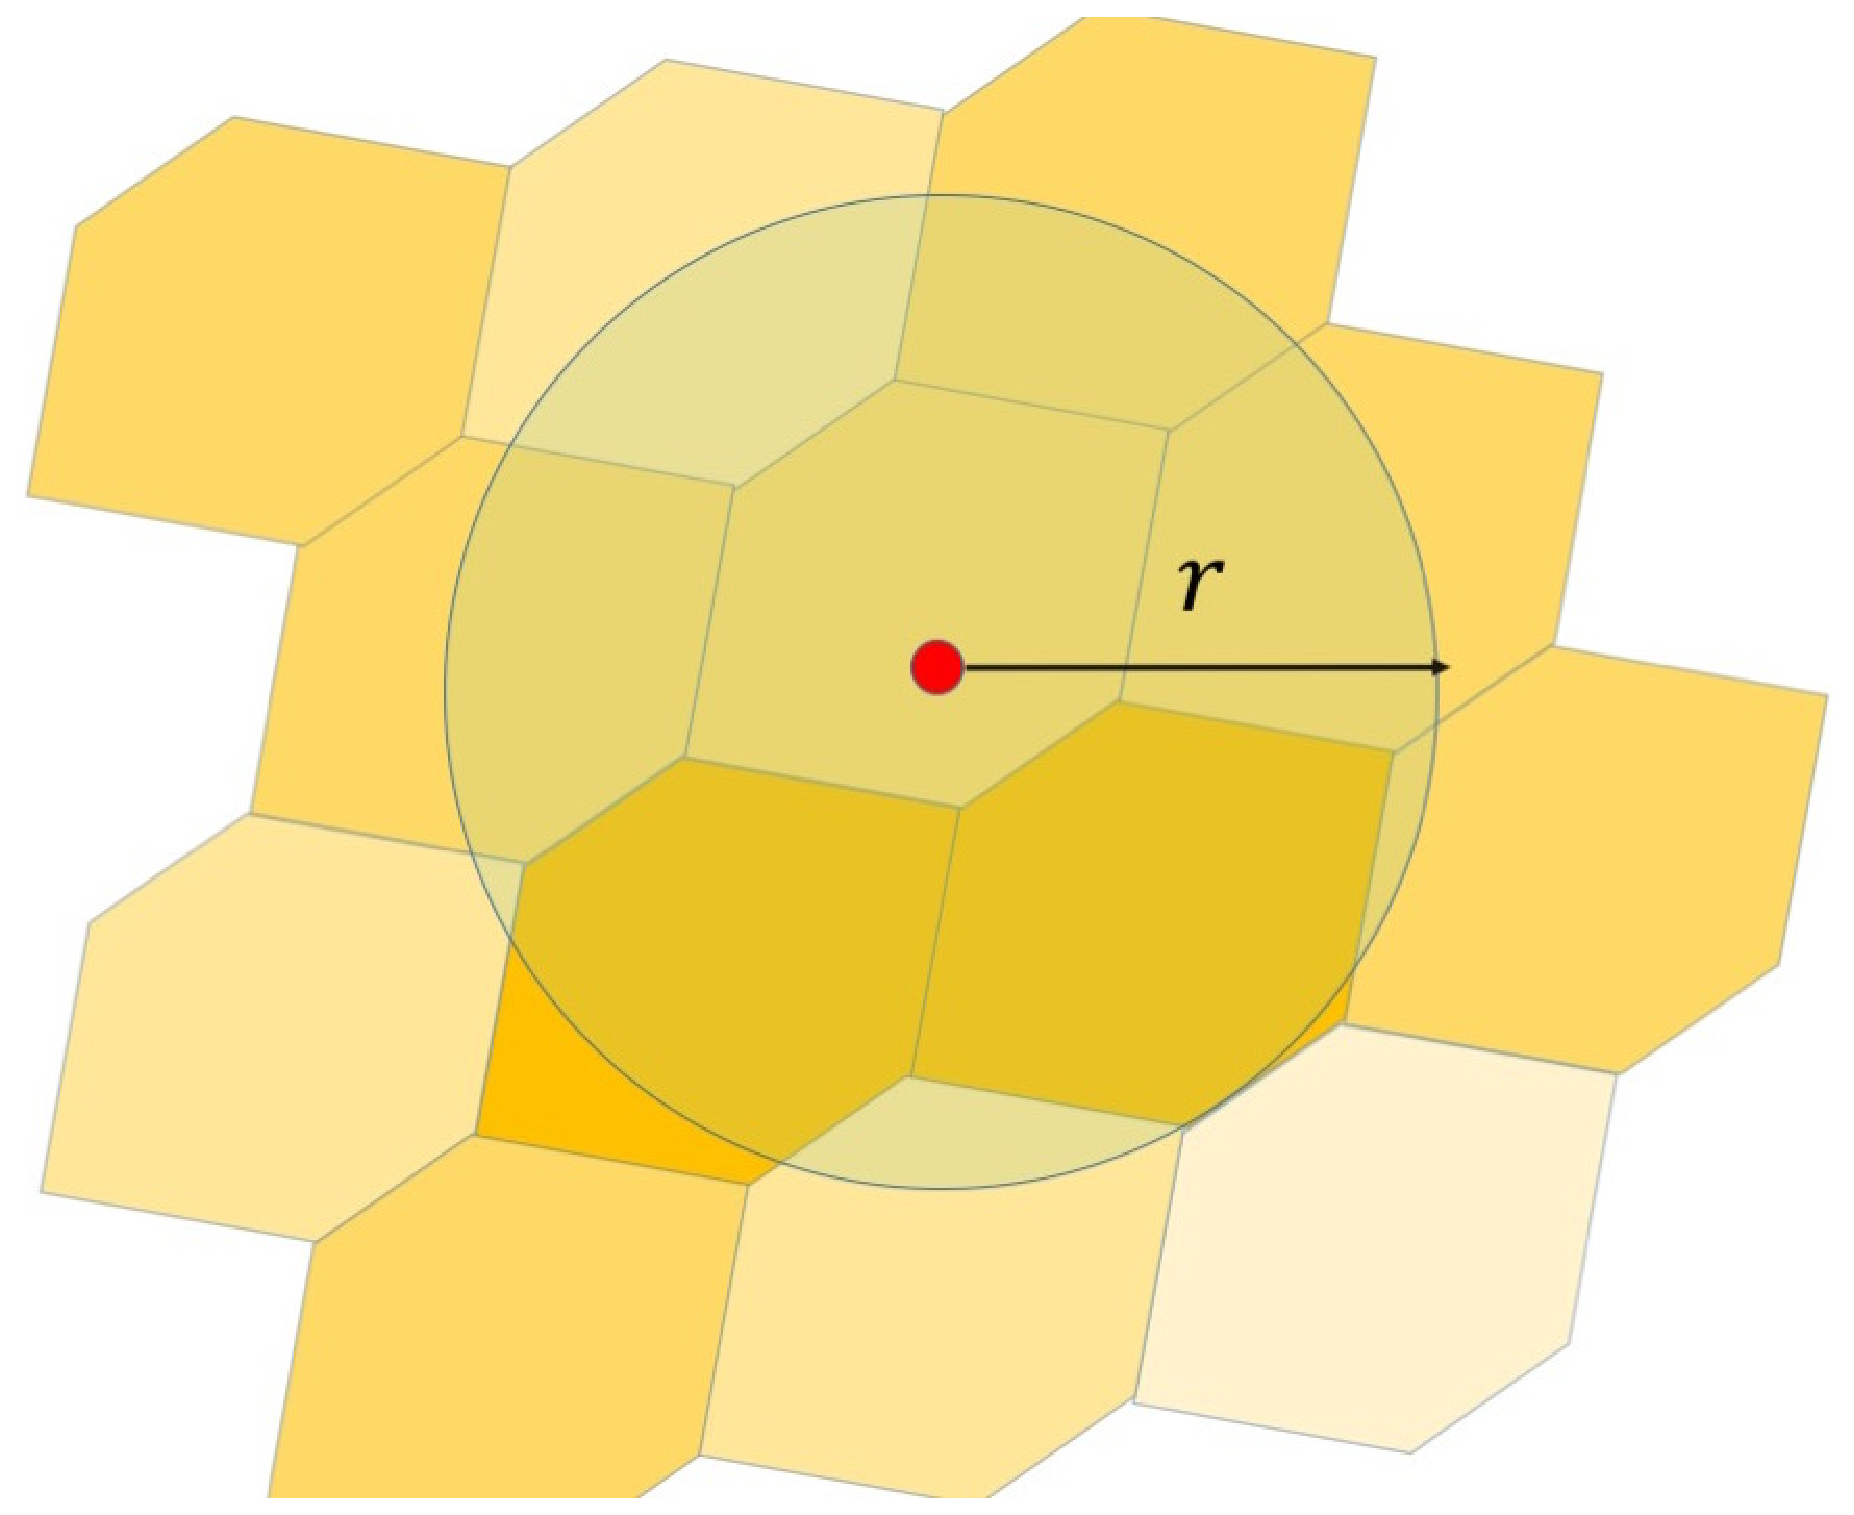
\includegraphics[width=1\textwidth]{images/buffer}
			\caption{In verde chiaro \`e rappresentato il buffer di raggio $r$ centrato  sull'edificio $b_i$. }
			\label{buffer}
		\end{minipage}
	\end{figure}
	
	\item \textbf{$ \mathcal{NZ}_i $ (Nearest Zones)} $ = \{nz_{i,j}(i=1,..,\mathbf{card}( \mathcal{B} )), (j=1,..,\mathbf{card}(\mathcal{ NZ}_i)) | nz_{i,j} \in  \mathcal{Z}  \cap HazardArea_i $ è una \textit{Nearest Zone}, ovvero 	una \textit{Zone} che si trova all'interno della $HazardArea_i$ di $b_i$\}. Gli $nz_{i,j}$ possono rappresentare le \textit{Zones} nella loro interezza, oppure parte di esse derivante dall'intersezione con la $HazardArea_i$.  (Figura \ref{NearestLand}).
	In seguito verrà usato sempre il pedice $\mathbf{j}$ accostato al pedice $\mathbf{i}$ per riferirsi alla nearest zone j-esima del building i-esimo.
	Nelle notazioni introdotte di seguito l'occorrenza del pedice $\{i,j\}$ viene usata $sempre$ per richiamare che ci si riferisce alla nearest zone $j-mo$ dell'edificio $i-mo$, ovvero all'elemento $nz_{i,j}$ di $ \mathcal{NZ}_i $.
	Si noti che $nz_{i,j}$ è una notazione sovraccaricata in quanto rappresenta sia l’\textit{ID} di una \textit{Nearest Zone} che la sua geometria.
	
	\item \textbf{$ cnz_{i,j} $ (Centroid of $nz_{i,j})$} corrisponde al centro di massa di $nz_{i,j}$ la cui posizione è descritta dalle sue coordinate geografiche (Figura \ref{cnz}). 
	
	\item \textbf{$ \mathcal{I} $} $ = \{i_p(p=1,2,..) | i_p $ \`e una \textit{isoipse} della GeoArea\}. Per isoipse si intende quella curva che unisce punti con uguale quota, descritta dalla tupla <\textit{ID}, \textit{elevation}, \textit{geometry}>. Il campo \textit{ID} identifica univocamente la curva di livello, \textit{elevation} la quota  e infine \textit{geometry} la geometria che descrive l'andamento dell'isoipse.
	
	\item \textbf{$ \mathcal{NI}_i $ (Nearest Isoipses)} $ = \{ ni_{i,o}(i=1,..,\mathbf{card}( \mathcal{B} )), (o=1,. . ,\mathbf{card}(\mathcal{ NI}_i)) | ni_{i,o} \in  \mathcal{I}  \cap HazardArea_i$ è la o-esima \textit{Nearest Isoipse} che si trova all'interno della $HazardArea_i$ di $b_i$ \}. Le $ni_{i,o}$ possono rappressentare le \textit{isoipse} nella loro interezza, oppure una parte di esse derivanti dall'intersezione con la $HazardArea_i$  (Figura \ref{NearestIso}). Si noti che $ni_{i,o}$ è una notazione sovraccaricata in quanto rappresenta sia l’\textit{ID} di una \textit{Nearest Isoipse} che la sua geometria.
	
	\begin{figure}[h]
		\hspace{0.05\linewidth}
		\begin{minipage}[t]{0.45\linewidth}
			\centering
			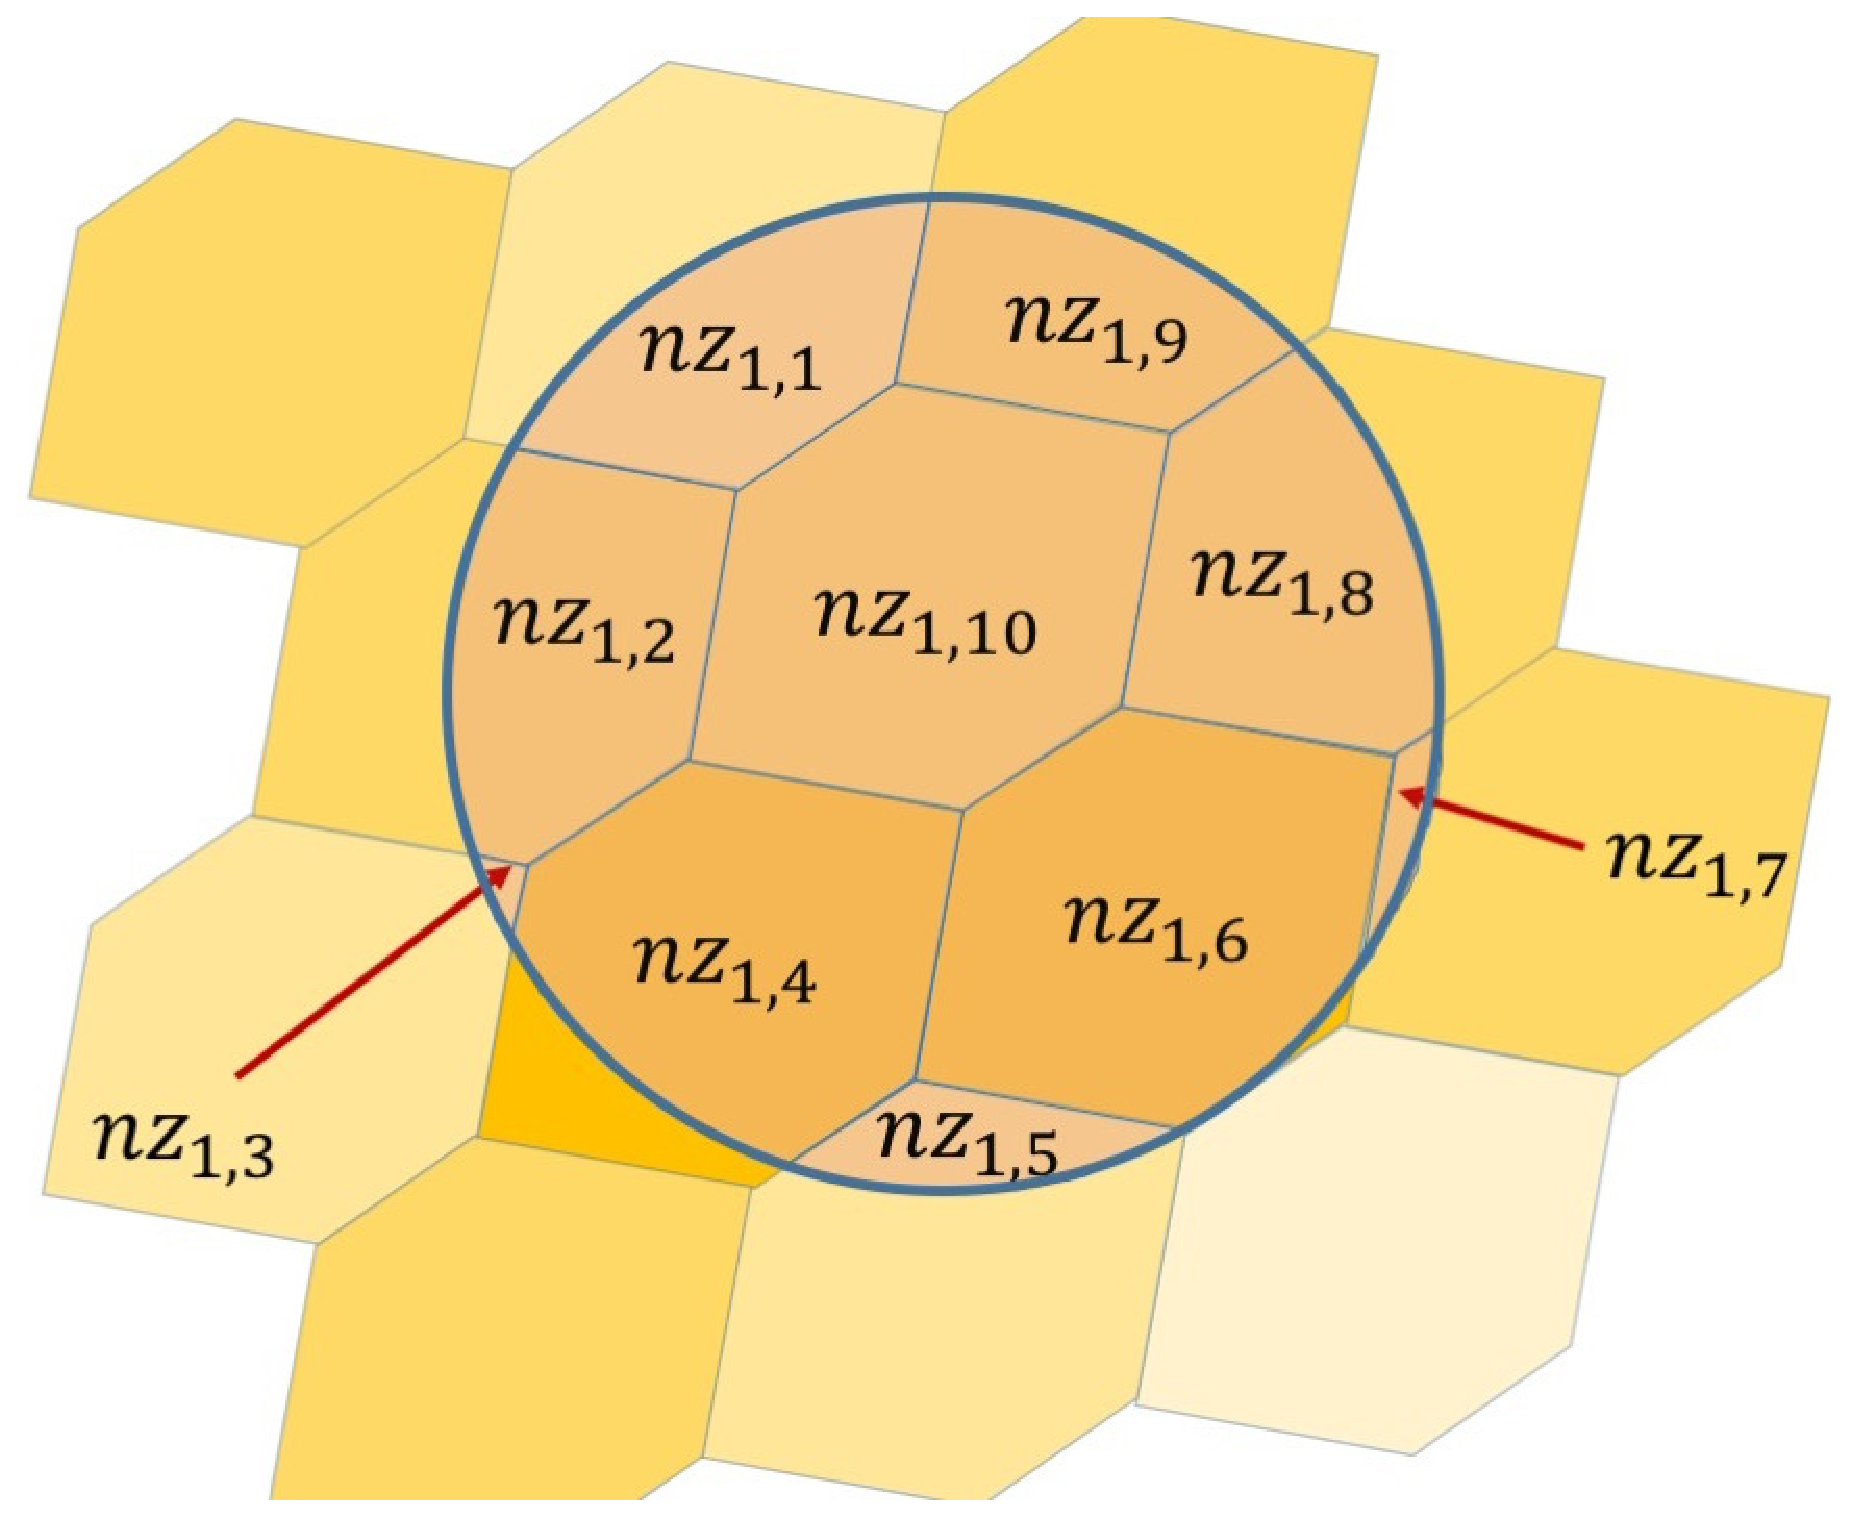
\includegraphics[width=1\textwidth]{images/NearestZone}
			\caption{In rosa sono rappresentate le $nz_{i,j}$ con $i=1$  che si trovano all'interno della $HazardArea_i$. E' possibile notare come $nz_{1,10}$ sia una \textit{Zone} intera mentre $nz_{1,3}$ è parziale.}
			\label{NearestLand}
		\end{minipage}
		\hspace{0.05\linewidth}
		\begin{minipage}[t]{0.45\linewidth}
			\centering
			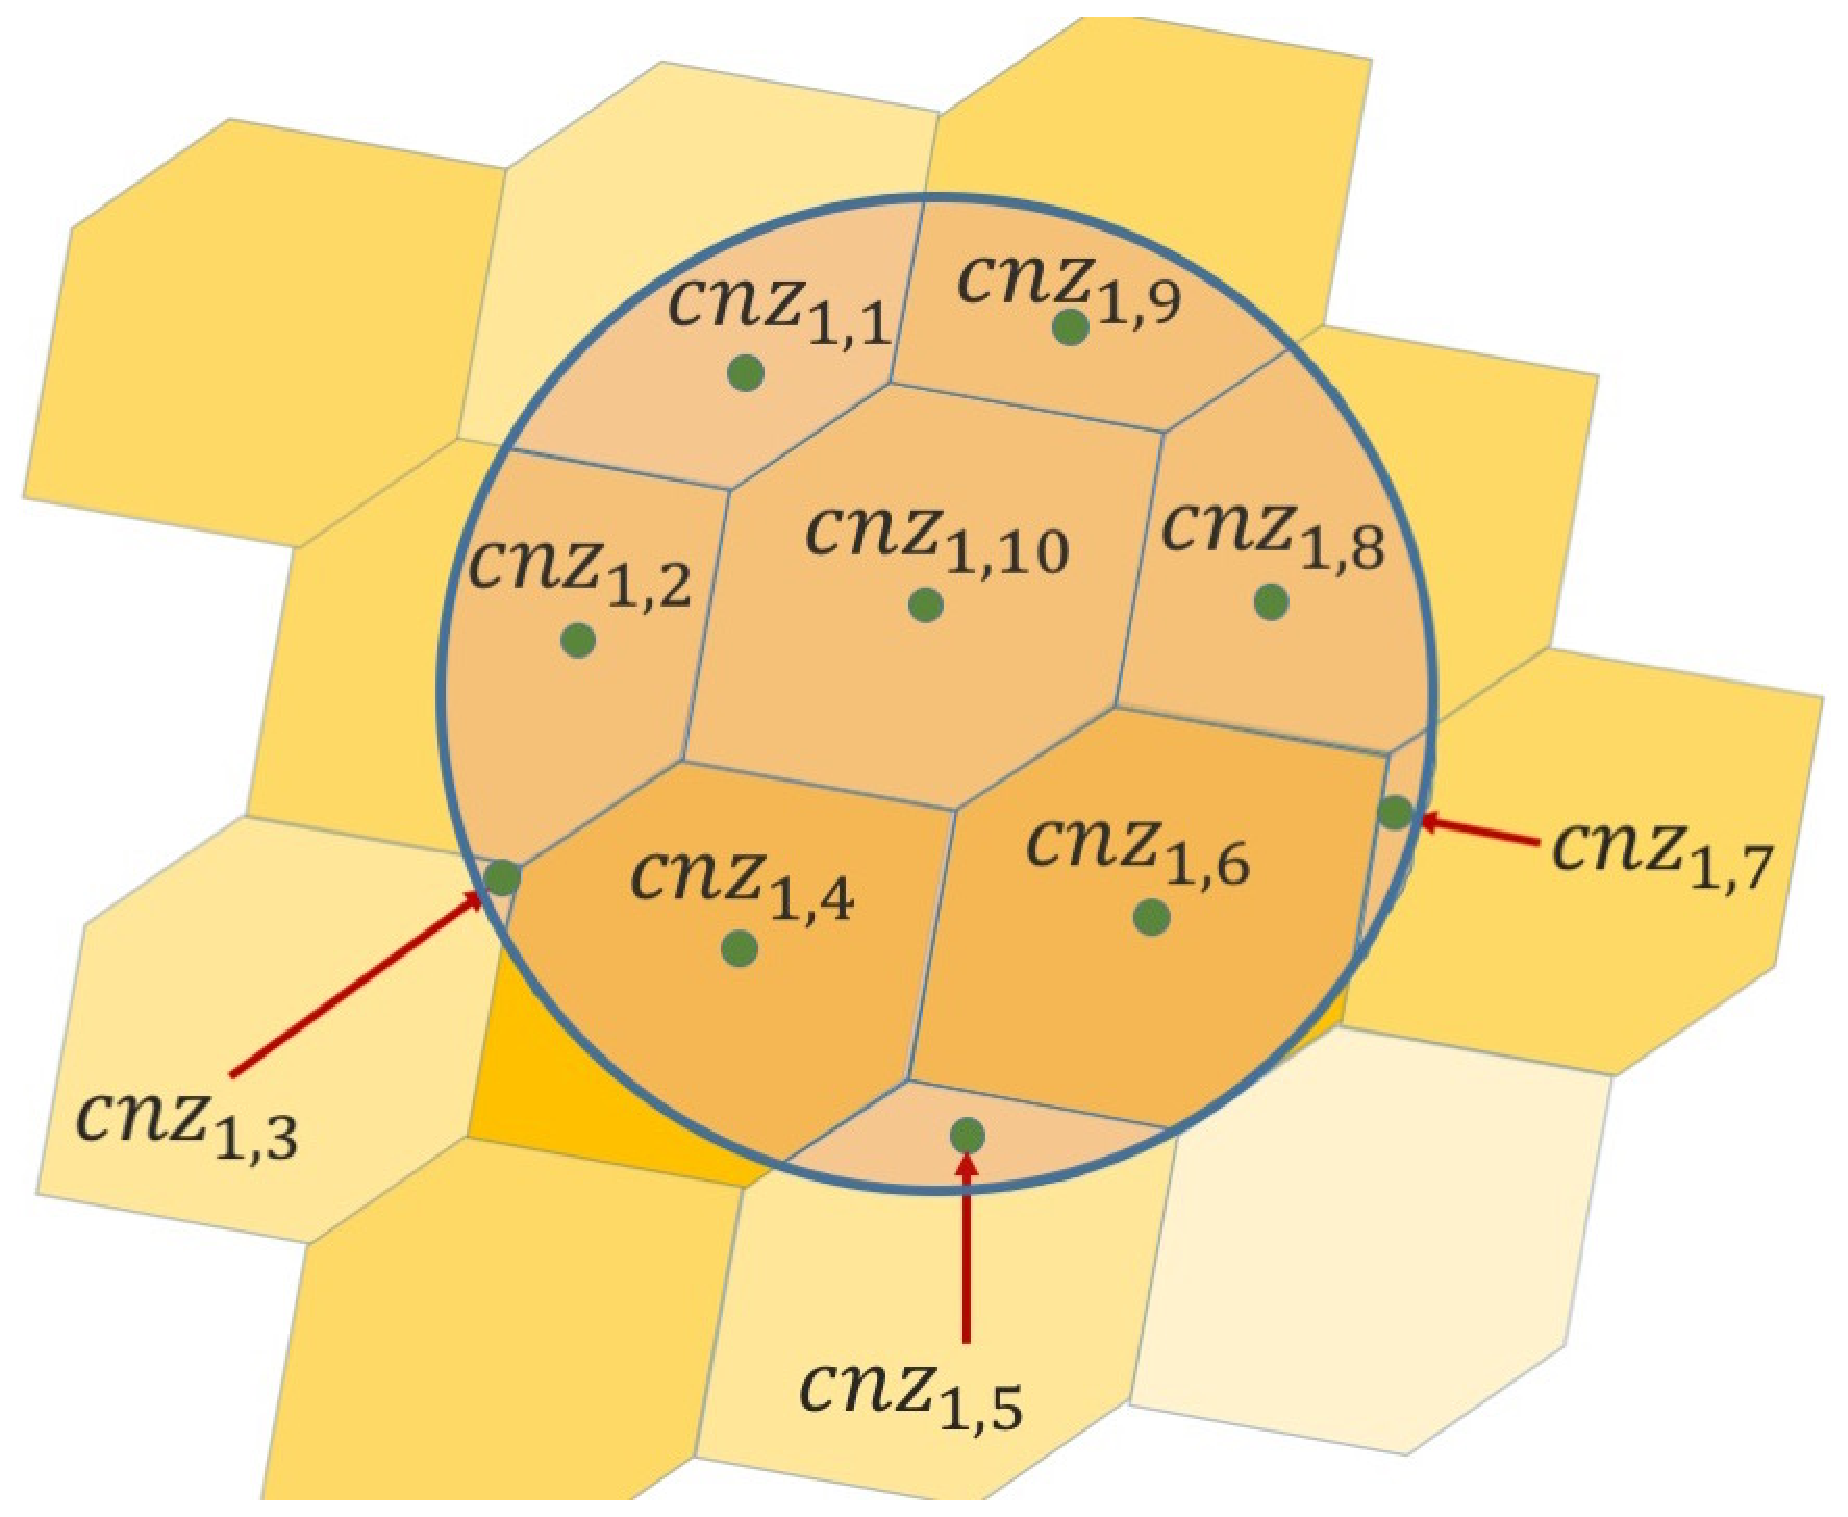
\includegraphics[width=1\textwidth]{images/cnz}
			\caption{Con i pallini verdi sono rappresentati i centri di massa $cnz_{i,j}$ degli $nz_{1,j}$.}
			\label{cnz}
		\end{minipage}
	\end{figure}
	
	\item \textbf{$\mathcal{ZF}_i$ (Zone Fragments)} $ = \{ zf_{i,j,t} (i=1,..,\mathbf{card}(\mathcal{B}),j=1,..,\mathbf{card}(\mathcal{NZ}_i),(t=1,..))| zf_{i,j,t}  $ è la t-esima \textit{Zone Fragment} interna alla nearest zone $nz_{i,j}$ restituita dall'operazione di splitting di detta nearest zone con le sole nearest isoipse in $\mathcal{NZ}_i $ che l'attraversa.
	I quattro poligoni in blu con i contorni gialli della Figura \ref{zf} rappresentano gli altrettanti \textit{Zone Fragments} nei quali la Nearest Zone $nz_{1,j}$ viene frammentata dall'operazione di split con le tre isoipse che la attraversano. $\mathcal{ZF}_i$ è l'insieme delle zone fragments prodotte dallo split tra gli $nz_{i,j} \in \mathcal{NZ}_i $ e le $ni_{i,o} \in \mathcal{NI}_i$ (Figura \ref{zf}). 
	
	
	\begin{figure}[h]
		\hspace{0.05\linewidth}
		\begin{minipage}[t]{0.40\linewidth}
			\centering
			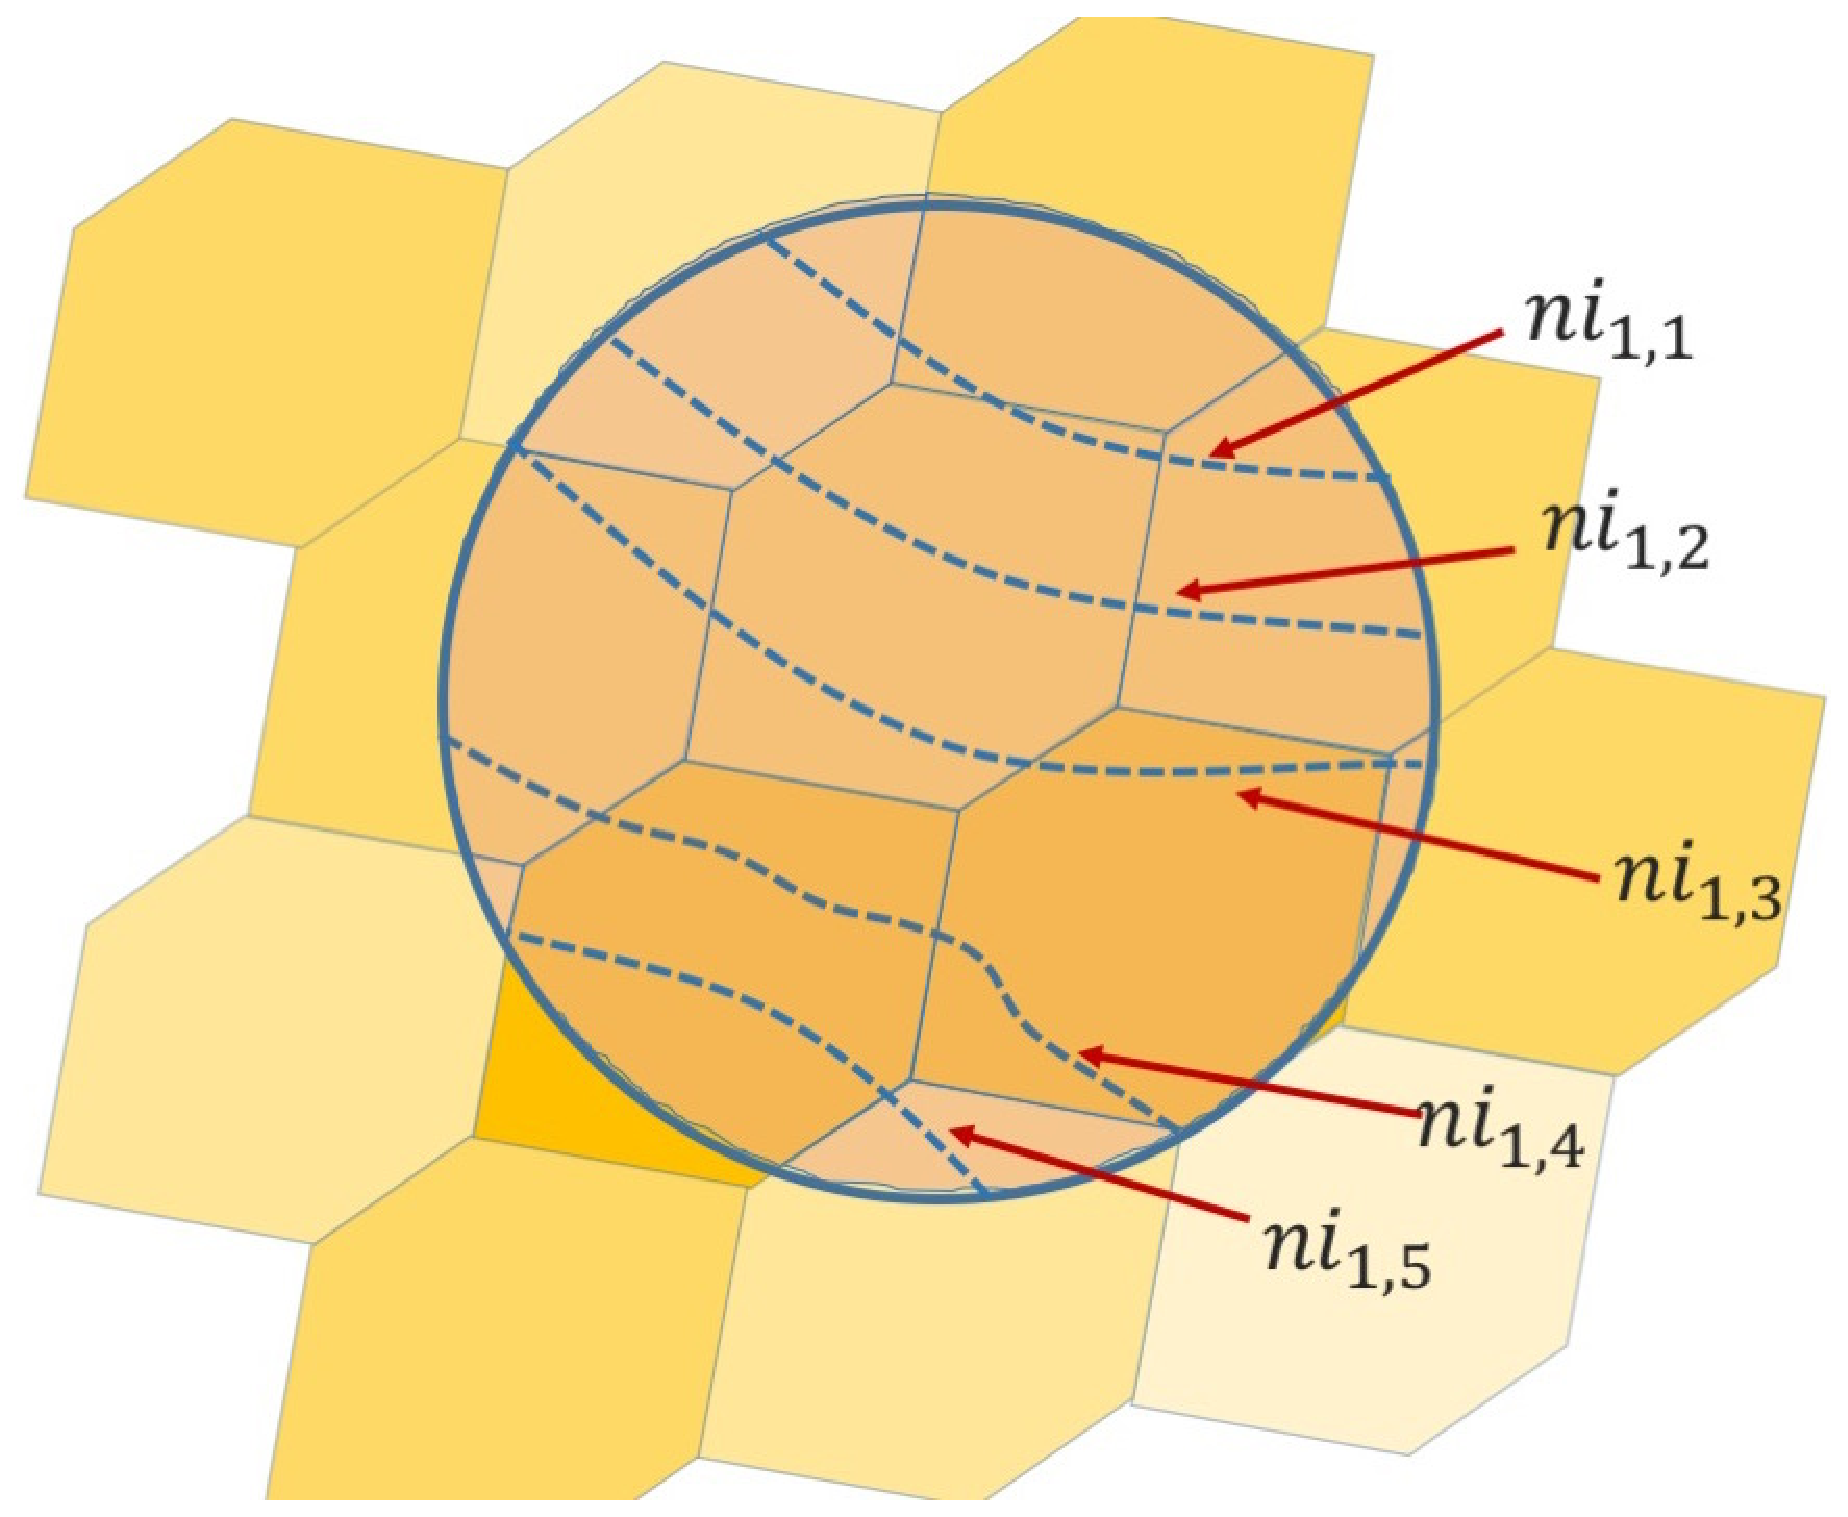
\includegraphics[width=1\textwidth]{images/ni}
			\caption{Le linee in blu tratteggiate rappresentano le nearest isoipse $ni_{1,o}$.}
			\label{NearestIso}
		\end{minipage}
		\hspace{0.05\linewidth}
		\begin{minipage}[t]{0.40\linewidth}
			\centering
			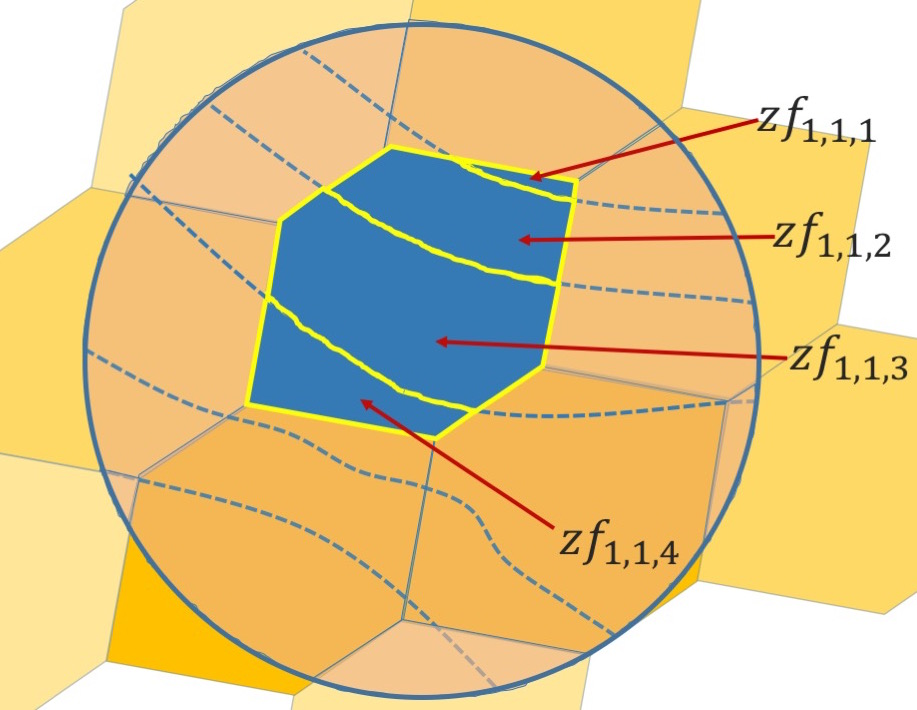
\includegraphics[width=1\textwidth]{images/zf}
			\caption{ 
				I quattro poligoni in blu con i contorni gialli rappresentano le $zf_{1,1,t}$ relative alla nearest zone $nz_{1,1}$. }
			\label{zf}
		\end{minipage}
	\end{figure}
	
	\item \textbf{ $czf_{i,j,t}$ (Centroid of $zf_{i,j,t})$} corrisponde al centro di massa dello zone fragment $zf_{i,j,t}$ la cui posizione è descritta dalle sue coordinate geografiche date dalla coppia $(czfx_{i,j,t}, czfy_{i,j,t})$ (Figura \ref{czf}).
	
	\begin{figure}[h]
		\centering
		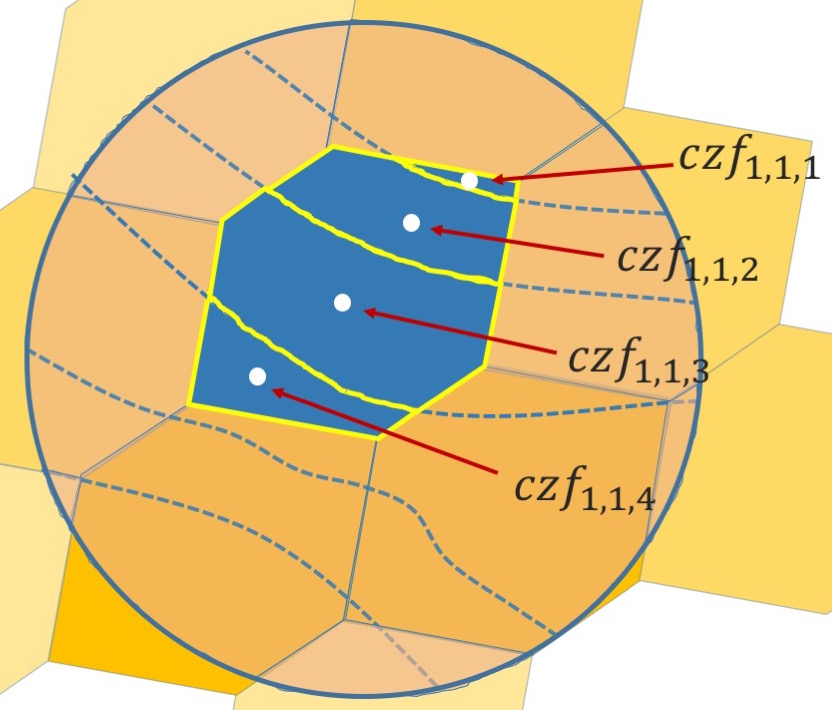
\includegraphics[width=0.40\textwidth]{images/czf}
		\caption{
			I pallini bianchi rappresentano i $czf_{1,1,t}$ ovvero i centri di massa delle zone fragments $zf_{1,1,t}$ della (Figura \ref{zf}) .}
		\label{czf}
	\end{figure}
	
	\item \textbf{$ \mathcal{LR}_i $} (\textbf{LinearRegressions}) $ = \{lr_{i,j}(i=1,..,\mathbf{card}(\mathcal{B})),(j=1,..,\mathbf{card}(\mathcal{NZ}_i)\} | lr_{i,j} $ rappresenta la retta di regressione lineare della \textit{Nearest Zone} $nz_{i,j}$. Nel caso specifico $lr_{i,j} $ rappresenta la retta passante per il centro di massa $cnz_{i,j}$ della nearest zone $nz_{i,j}$ con coefficiente angolare \textit{m} tale che, dati i centri di massa ($czfx_{i,j,t}, czfy_{i,j,t}$)  delle zone fragment $zf_{i,j,t}$,  sia minima la somma dei quadrati dei loro scarti (Figura \ref{linear_regression}). Matematicamente essa è descritta come segue:\\
	\\
	l'equazione (\ref{eq:retta_passante_per}) rappresenta la retta passante per il centro di massa $cnz_{i,j}$ rappresentata in Figura \ref{linear_regression}
	\begin{equation}\label{eq:retta_passante_per}
		y - cnzy_{i,j} = m(x-cnzx_{i,j})
	\end{equation}
	
	per la quale dati $t$ punti ($czfx_{i,j,t}, czfy_{i,j,t}$) risulta minima la somma dei quadrati degli scarti:
	\begin{equation}\label{eq:somma_degli_scarti}
		S(m, q) = \sum_{i=0}^n (m*czfx_{j,t} + q - czfy_{j,t})^2 
	\end{equation}
	\begin{equation}
		\textnormal{ove}\: q = cnzy_{i,j} - m*cnzx_{i,j}
	\end{equation}
	Questo concetto matematico sarà utilizzato per stimare la direzione di caduta della frana relativa alla $nz_{i,j}$ Figura \ref{linear_regression}.
	
	
	\begin{figure}[h]
		\centering
		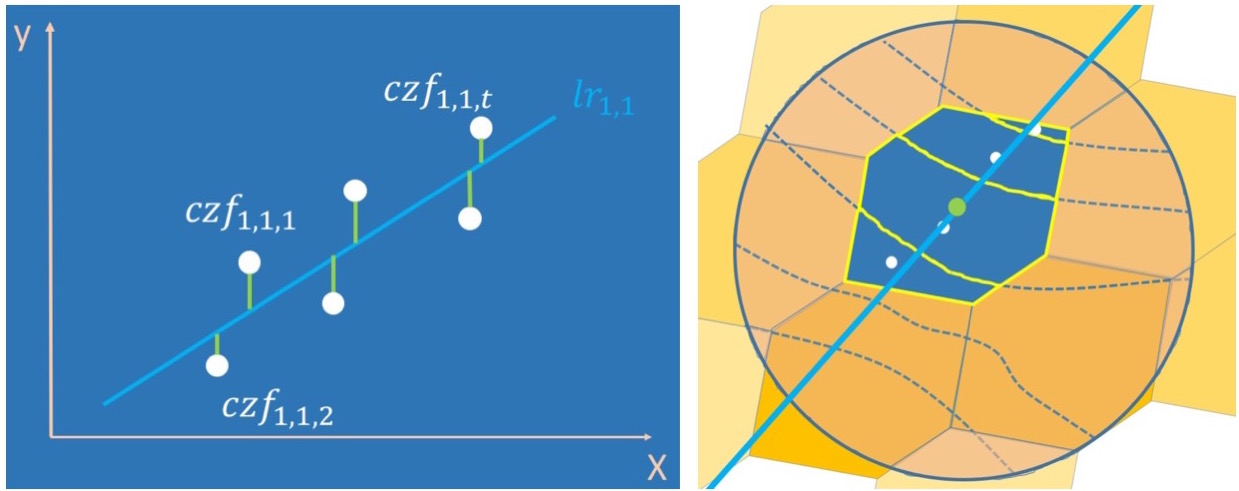
\includegraphics[width=0.8\textwidth]{images/linear_regression}
		\caption{La retta di regressione lineare $lr_{i,j}$ di colore celeste, minimizza la distanza (rappresentata con la linea verde chiaro) tra i punti (in questo caso gli $czf_{i,j,t}$) e la retta stessa.}
		\label{linear_regression}
	\end{figure}
	
	\item \textit{$BuildingBuffer_i$} rappresenta l'area circostante l'edificio $b_i$ e ne approssima l'estensione. E' definita come la circonferenza centrata su $b_i$ di raggio $l$ dove $l<<r $ con $r$ raggio del \textit{$HazardArea_i$} (Figura \ref{buildingimpactfactor}).
	
	\begin{figure}[h]
		\centering
		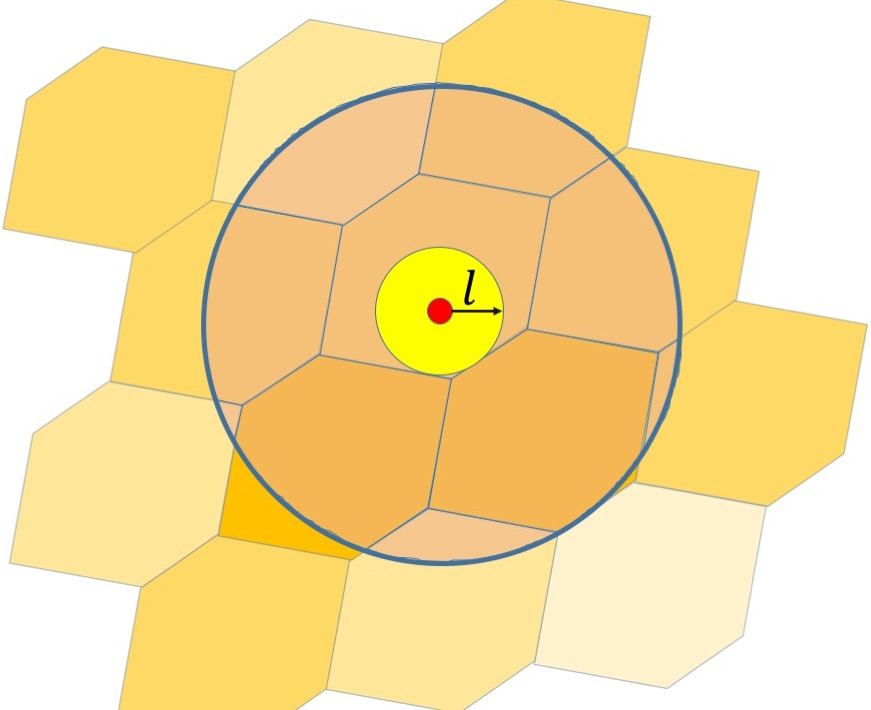
\includegraphics[width=0.5\textwidth]{images/buildingimpactfactor}
		\caption{\textcolor{red} {(L'immagine deve avere l al posto di d)} L'area di colore giallo intorno all'edificio rappresenta il $BuildingBuffer_i$ di raggio $l$.}
		\label{buildingimpactfactor}
	\end{figure}
	
	\item \label{last_enum} \textbf{$EXP$ (Exposure)} $ = \{exp_i(i=1,..,\mathbf{card}(\mathcal{B})) | exp_i $ è il valore di \textit{exposure} del building i-esimo. Per \textit{exposure} si intende il valore numerico che indica quanto il building è esposto al rischio frana, 
	rappresentato dalla tupla <\textit{ID}, \textit{description}, \textit{position}, \textit{exposure}> 
	
\end{enumerate}
